\documentclass[../synthesisAndCharacter.tex]{subfiles}
\graphicspath{{\subfix{../../../images/}}}
\begin{document}
    \textbf{Annealing} is a heat treatment process that involves heating a material to a specific temperature and holding 
    it at that temperature for a certain period, followed by controlled cooling. The purpose of annealing is to 
    modify the material's properties, such as its microstructure, mechanical strength, electrical conductivity, 
    and thermal stability. Annealing is widely used in various fields, including metallurgy, materials science, 
    and semiconductor manufacturing. During the annealing process, several changes occur within the material:
    \begin{Figure}
        \centering
        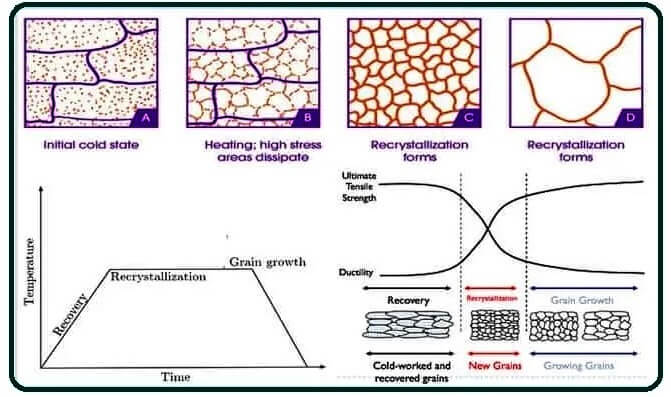
\includegraphics[width=0.8\linewidth]{annealing.jpg}
        \captionof{figure}{Various stages of annealing\cite{u9}}\label{fig:annealing}
    \end{Figure}
    \begin{itemize}
        \item \textbf{Recrystallization:} Annealing promotes the formation of new, defect-free crystals within the 
        material. It helps eliminate dislocations and other crystal defects that may have occurred during 
        processing or deformation, leading to the growth of larger, more regular grains.
        \item \textbf{Stress Relief: } Annealing helps relieve internal stresses within the material, which can 
        result from processes like casting, forming, or rapid cooling. By heating the material to a specific 
        temperature and holding it there, the internal stresses can be reduced, leading to improved dimensional 
        stability and reduced risk of cracking or distortion.
        \item \textbf{Grain Growth: }Annealing allows for the controlled growth of grains within the material. 
        This is particularly important in polycrystalline materials, where larger grains can enhance mechanical 
        properties, such as strength and toughness.
        \item \textbf{Phase Transformation: }In some cases, annealing induces phase transformations within the 
        material, leading to changes in its composition and crystal structure. This can result in the formation 
        of desired phases with improved properties
    \end{itemize}
\end{document}